%!TEX root = thesis.tex
\chapter{Data-wise Opportunistic Routing with Spatial Information}
\label{DORSI}
% \SVN $Revision: 838 $
% \SVN $Author: sgordon $
% \SVN $Date: 2014-05-12 13:30:42 +0700 (Mon, 12 May 2014) $
% \SVN $URL: https://sandilands.info/svn/Common/Styles/siitthesis/chapter4.tex $

Opportunistic Network (OppNet), a subclass of Delay/Disruption-Tolerant Network (DTN), is a network paradigm that the communication contacts are intermittent. This challenged network which is also referred as Intermittently Connected Mobile Network (ICMN), is involving mobile nodes to communicate with each other without existing complete end-to-end path from source to destination. Traditional routing protocols have been exhibited ineffective in coping with unreliable and unpredictable wireless medium \cite{Yang2009} since they implicitly assume that the network is connected and an end-to-end path always exists between any source and destination. This conventional infrastructure network commonly utilizes the network topology to route the message, thus it presents inadequate performance in highly dynamic topological environment. In such extreme condition such as military tactical network, DTN and Mobile Ad-hoc Network (MANET) are among several promising challenged researches aiming to improve network performance. DTN protocols typically address sparse intermittently connected networks whereas MANET protocols address the fairly stable and fully connected ones. However, many intermediate situations may occur on mobility dynamics or radio link instability. In such cases, where the network frequently splits into evolving connected groups, none of the conventional routing paradigms are fully satisfactory \cite{Whitbeck2010}. To address the problem of intermittent links and node mobility, local forwarding are exploited in order to transfer the messages. The opportunistic routing pattern, called store-carry-forward, takes an advantage of node mobility to forward the data buffered in the carried node to the next connected node during the opportunistic contacts. Basically, the terms opportunistic networks and delay tolerant networks are occasionally used interchangeably. DTN usually computes the estimation of delivery delays in advance due to some degree of determinism of system variables. On the other hand, opportunistic link in OppNet is highly dynamic and unpredictable so routes are computed at each hop when forwarding messages \cite{Bujari2012a}. This network scheme is suitable for extreme dynamic evolving network topology and limited information scenarios. The applications of opportunistic network is typically used in an environment that is tolerant of long delay and high error rate such as MANET in battlefield communication \cite{Alspaugh2004} or DTN for interplanetary networking \cite{Jenkins2010}. Routes in opportunistic network are built dynamically based on knowledge about topological evolution of the network. Routing performance improves when acquiring
more knowledge about the expected network topology. Nevertheless, a tradeoff between performance and knowledge requirement must be met since this kind of knowledge is difficult to acquire. If the knowledge is not available or difficult to achieve, epidemic routing (context-oblivious) might be the best option for communication \cite{bonaldo2011}.

Even though, this flooding based routing tends to minimize the latency, it consumes network resource and tends to degrade performance. Most of the existing routing schemes for opportunistic network rely on a priori knowledge topology information \cite{Pelusi2006}, especially focusing on the dissemination algorithms and policy to control or limit flooding \cite{Plymoth2010}.

In this chapter, we present a routing protocol in opportunistic environment that dynamically prioritizes the candidate messages based on the content of the data. Since security is an increasing concern in military and other critical operation mission, it is vital to route data of different sensitivities differently. The most significant and sensitive data should be guaranteed its higher level of delivery and protection than common data. However, only few works have applied the well-defined information sensitivity concept such as Multi Level of Security (MLS) \cite{Kotrappa2010,marking2010} to network information such as routing information, QoS signaling and other management information \cite{Winjum2008}.

In this routing scheme, we purpose to incorporate the information sensitivity concept into the messages in order to route the data differently in compliance with the classes of messages. To the best of our knowledge, this method has not been fully explored in the existing literatures. In this research, we extend our previous work \cite{Kerdsri2012} by generalizing information sensitivity parameters and involving spatial information into routing decision to improve the network efficiency. We conducted Opportunistic Network Environment (ONE) simulation \cite{Keranen2009b} to evaluate the performance of DORSI protocol.

%=============================================================================
\section{Opportunistic network model}
\label{DORSI:Opportunistic network model}
%=============================================================================

\begin{figure}[!t]
\centering
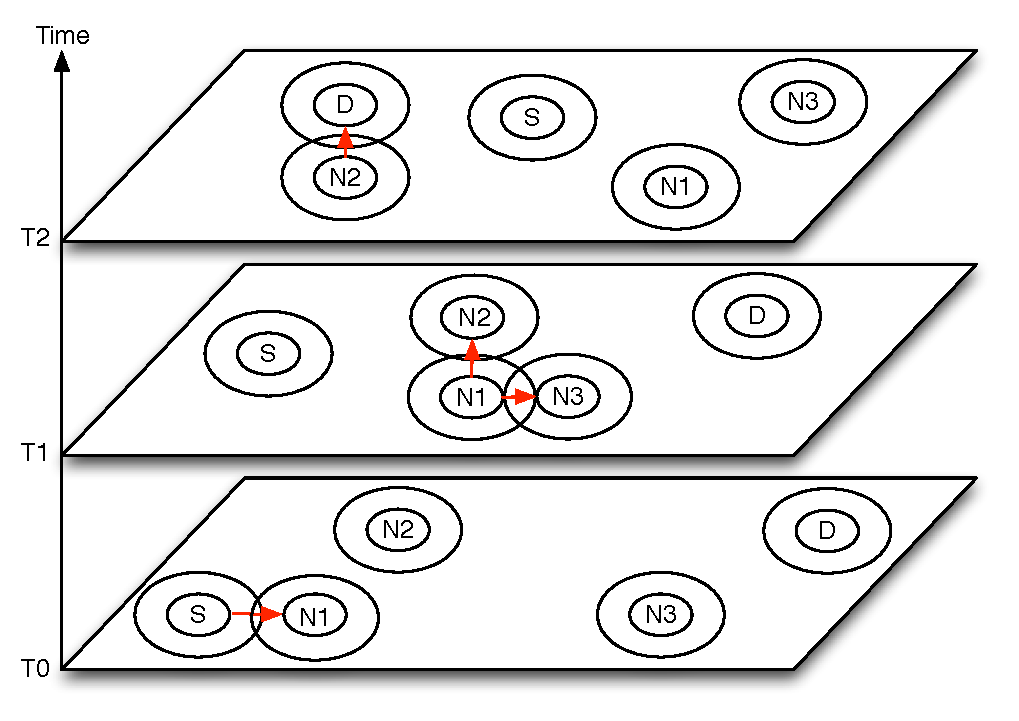
\includegraphics[width=5in]{Figures/OpportunisticNetworkNodel.pdf}
\caption{Opportunistic network model}
\label{Opportunistic network model}
\end{figure}

Since opportunistic network commonly operates in multi-hop wireless ad-hoc network environment, links may be disrupted or shut down periodically when nodes move away or absent which resulting in intermittent connectivity \cite{Moreira2011}. As a result, nodes require to communicate with each other via opportunistic contacts through store - carry - forward fashion \cite{Chung-Ming2008}. Instead of selecting a node to act as the next hop, multiple relay nodes may be determined when a data packet is being transmitted. This decision is carried out for each data packet according to the instantaneous wireless links condition in order to select the best relaying nodes. In OppNet, a node is an entity acting as a host, router or gateway. Each node can route and exchange message (full-duplex) between nodes that move randomly among remote fragment of network within its contact period. Nevertheless, OppNet node must contain enough processing power and storage to keep the data until this node gets contact with intermediate carrier or destination node. Within this disruptive environments, the contact period is extremely dynamic since contact may appear arbitrarily without prior information and this transmission link can be absent at any time.

Fig. \ref{Opportunistic network model} presents the model of OppNet routing exploiting their node mobility and contacts for data delivery. A node can exchange message with other intermediate nodes inside its wireless coverage area until the message reach the destination. From Fig. \ref{Opportunistic network model}, all node can move with time (T0 - T2 as an example). At T0, The source node transmit the data to the next node within its radio coverage. This receptors at T1 now can act as a relay node and replicate message to the other nodes in its wireless link radius until this message reach the final destination at T3. Therefore, OppNet leads to a load balancing while it increases the robustness of the multi-hop wireless network as multiple receptors are potential relays.


%=============================================================================
\section{DORSI routing algorithm}
\label{DORSI:DORSI routing algorithm}
%=============================================================================
\begin{figure}[!t]
\centering
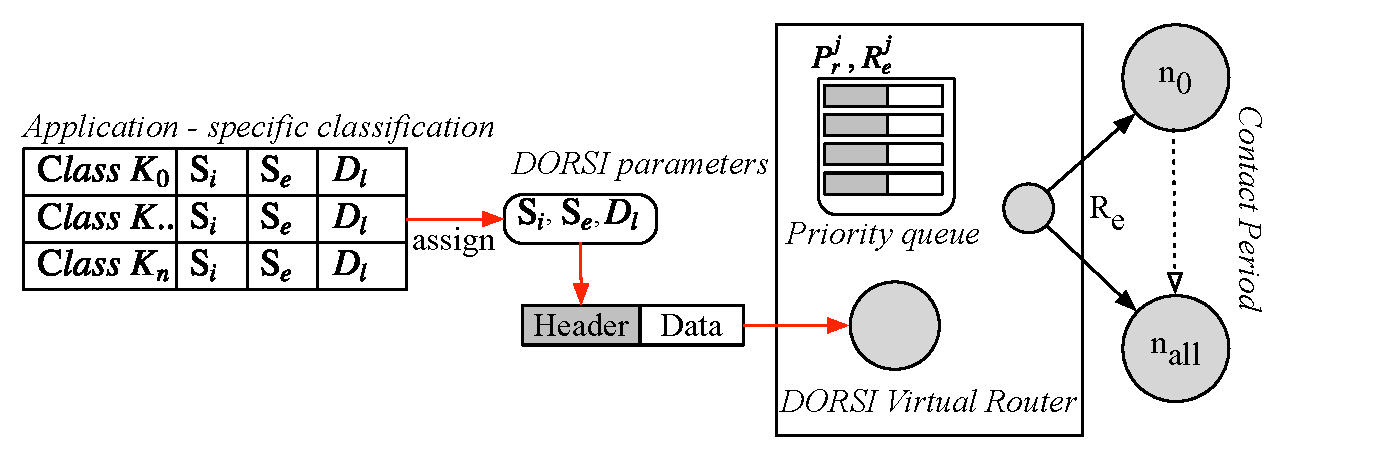
\includegraphics[width=5in]{Figures/DORSIsystemModel.pdf}
\caption{DORSI system model}
\label{DORSI system model}
\end{figure}

The design goal of DORSI is to distinguish the data with different information sensitivity concept. 
%%
We implement this protocol in order to guarantee that the important message can reach the destination within the time limit resulting in higher delivery ratio. 
%%
Additionally, we need to control the security risk of the message with higher security level by limiting the number of message replica in this network according with information sensitivity concept \cite{Kotrappa2010,marking2010}. 
%%
The final goal of this protocol is to increase the bandwidth efficiency by selecting the candidate nodes with higher probability of delivering the message to the destination.

Fig. \ref{DORSI system model} shows the proposed DORSI system model implemented as a virtual (software) router in an OppNet node. 
%%
In DORSI, besides common routing information such as source and destination addresses, every delivered message is associated with 3 additional DORSI parameters which are Significant level ($S_i$) Security level ($S_e$), Delivery deadline ($D_l$). 
%%
The $S_i$ represents how important of this message while the $S_e$ defines the level of this data that needs to be protected. 
%%
The $D_l$ element is the message expiration time. 
%%
If the delivery deadline is reached, the message will be dropped. 
%%
The value of these DORSI parameters are determined in accordance with the application specific requirement. 
%%
For example, the contents in military domain are divided into several classifications based on the multilevel of security which is intended to prevent unauthorized personnel from accessing information at higher classification than their authorization \cite{Winjum2008}. 
%%
Therefore, different classes of message in military perspective are treated differently.


At DORSI router, a time-constrained priority queue is used to carry DORSI messages waiting for being forwarded to the next node. 
%%
The DORSI parameters: $S_i$ , $S_e$ and $D_l$ are used in routing decision of DORSI virtual router on a node when this node opportunistically contacts to the other nodes. 
%%
Upon node contact, messages will be processed orderly according to their up-to-date priority value, however the message whose delivery deadline is reached will not be considered and will be removed out of the queue. 
%%
The priority value ($P_r^j$) of a specific message, $j$, is calculated based on its significant level and its expediting factor, $\xi(D_l^j, t)$, as in Eq. \ref{Eq:DORSI:routing algorithm}

\begin{eqnarray}
\label{Eq:DORSI:routing algorithm}
{ P }_{ r }^{ j }={ w }_{ p }{ S }_{ i }^{ j }+(1-{ w }_{ p })\xi ({ D }_{ l }^{ j },t)
\end{eqnarray}

where

\begin{equation*}
 \xi ({ D }_{ l }^{ j },t)=\begin{cases} 0;{ \tau  }_{ t }>{ \tau  }_{ max } \\ \frac { { \tau  }_{ max }-{ \tau  }_{ t } }{ { \tau  }_{ max }-{ \tau  }_{ min } }  \\ 1;{ \tau  }_{ t }<{ \tau  }_{ max } \end{cases};{ \tau  }_{ min }\le { \tau  }_{ t }\le { \tau  }_{ max } 	
\end{equation*}

The $W_p$ level and expediting factor components.
%%
We define $\tau_t$ as residual lifetime of message which is calculated from $D_t^j - t$. 
%%
The expediting factor value, in the range [0,1], is composed from the message
residual lifetime, compared with the maximum and minimum countable message lifetime, $\tau_{max}$ and $\tau_{min}$, in the system. 
%%
The message with the residual lifetime $\tau_t$ = $\tau_{max}$ is considered as no need to expedite the message delivery while the message with $\tau_{min}$ is considered for maximum expediting.
%%
Note that the $P_r^j$ value will be recalculated at every time any node get contacted. 
%%
When a specific message,$j$ , is being processed, the determination whether it should be copied and sent to a specific contact node is controlled by the replication probability value, $R_j^e$, calculated at a contact time as in Eq. \ref{Eq:DORSI:replication probability}.


\begin{eqnarray}
\label{Eq:DORSI:replication probability}
{ R }_{ e }^{ j }=(1-{ R }_{ min })[{ w }_{ r }{ P }_{ r }+(1-{ w }_{ r })(1-{ S }_{ e }^{ j })]+{ R }_{ min }
\end{eqnarray}

The replication probability value, in range of [${ R }_{ min }$, 1], is based on the concept that a message with
more priority, $P_r^j$, should be disseminated more in order to increase delivery ratio while the message with more security level should be replicated less in order to tighten security risk. 
%%
In the formula, the replication weight coefficient, $w_r$ , is used to balance effect between both components. 
%%
The ${ R }_{ min }$ is the minimum guaranteed replication probability value in the system so that even a message with very low priority and very high security still has a chance to be forwarded. 
%%
This ${ R }_{ min }$ is a configurable system parameter according to application requirement.
In case that there are several nodes simultaneously contacts when processing a specific message, the node with higher rank will be considered before the lower one. 
%%
The ranking value of a contacting node, 𝑛, is calculated according to its departure probability representing the relative chance to move away from the DORSI router node, $r$.

\begin{eqnarray}
\label{Eq:DORSI:node ranking model}
{ N }_{ r }^{ n }=\sqrt { { ({ x }_{ n }\cos { { \theta  }_{ n } } -{ x }_{ r }^{ t }\cos { { \theta  }_{ r }^{ t } } ) }^{ 2 }-{ ({ y }_{ n }\sin { { \theta  }_{ n } } -{ x }_{ r }^{ t }\sin { { \theta  }_{ r }^{ t } } ) }^{ 2 } } -\sqrt { { ({ x }_{ n }-{ x }_{ r }^{ t }) }^{ 2 }-{ ({ y }_{ n }-{ x }_{ r }^{ t }) }^{ 2 } } 
\end{eqnarray}

It can be estimated as the difference in distance between the current DORSI router, $r$, and the contacting node $n$ , after they moves further one unit distance in their current direction. 
%%
Given that the positions of the router 𝑟 and the contacting node 𝑛 are (𝑥𝑟,𝑦𝑟) and (𝑥𝑛,𝑦𝑛). In addition, their moving
⃗⃗ ⃗⃗⃗⃗
direction vectors are 𝑑𝑟 = 𝑐𝑜𝑠𝜃𝑟𝑥̂ + 𝑠𝑖𝑛𝜃𝑟𝑦̂𝑎𝑛𝑑 𝑑𝑛 = 𝑐𝑜𝑠𝜃𝑛𝑥̂ + 𝑠𝑖𝑛𝜃𝑛𝑦̂, respectively. The ranking
value, 𝑁𝑟𝑛 is defined by formula in Eq. \ref{Eq:DORSI:node ranking model}. The positive 𝑁𝑟𝑛 value means the contacting node is moving away while the negative value means that it becomes closer. The contacting node with higher 𝑁𝑟𝑛 is needed to be considered since there is higher probability that it will be out of reach soon, compared with the other nodes. In Fig. \ref{Eq:DORSI:node ranking model}, 𝐷0 represents the distance between node 𝑟 and 𝑛 at time 𝑡 = 0 while 𝐷1 is a distance at the time t=1. If 𝐷1 > 𝐷0 , both nodes tend to move away from each other which results in higher node ranking.

Note that all messages where lifetime reach their deadline are discarded from the carried node. In addition, DORSI node will not receive the same copy of a specific message.

\begin{figure}[!t]
\centering
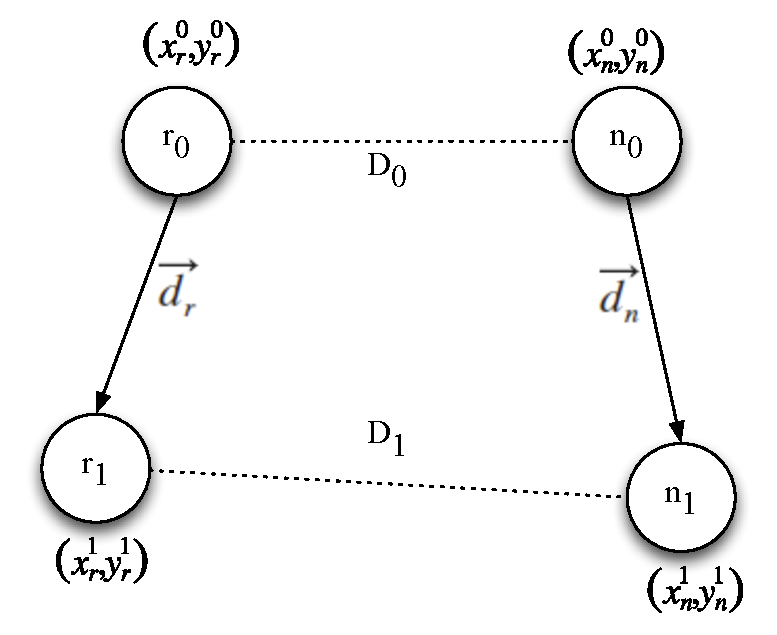
\includegraphics[width=5in]{Figures/NodeRankingModel.pdf}
\caption{Node ranking model}
\label{Node ranking model}
\end{figure}

%=============================================================================
\section{Summary of Contributions}
\label{DORSI:Summary of Contributions}
%=============================================================================



















































